\documentclass[a4paper,14pt,oneside,final]{extarticle}
\usepackage[top=2cm, bottom=2cm, left=3cm, right=1cm]{geometry}
\usepackage{scrextend}

\usepackage[T2A,T1]{fontenc}
\usepackage[ukrainian,russian,english]{babel}
\usepackage{tempora}
\usepackage{fontspec}
\setmainfont{tempora}

% Зачем: Отключает использование изменяемых межсловных пробелов.
% Почему: Так не принято делать в текстах на русском языке.
\frenchspacing

\usepackage{indentfirst}
\setlength{\parindent}{1.25cm}
\renewcommand{\baselinestretch}{1.5}

% Header
\usepackage{fancyhdr}
\pagestyle{fancy}
\fancyhead{}
\fancyfoot{}
\fancyhead[R]{\small \selectfont \thepage}
\renewcommand{\headrulewidth}{0pt}

% Captions
\usepackage{chngcntr}
\counterwithin{figure}{section}
\counterwithin{table}{section}
\usepackage[tableposition=top]{caption}
\usepackage{subcaption}
\DeclareCaptionLabelFormat{gostfigure}{Рисунок #2}
\DeclareCaptionLabelFormat{gosttable}{Таблиця #2}
\DeclareCaptionLabelSeparator{gost}{~---~}
\captionsetup{labelsep=gost}
\captionsetup[figure]{labelformat=gostfigure}
\captionsetup[table]{labelformat=gosttable}
\renewcommand{\thesubfigure}{\asbuk{subfigure}}

% Sections
\usepackage[explicit]{titlesec}
\newcommand{\sectionbreak}{\clearpage}

\titleformat{\section}
  {\centering}{\thesection \quad}{0pt}{\MakeUppercase{#1}}
\titleformat{\subsection}[block]
  {\bfseries}{\thesubsection \quad #1}{0cm}{}

\titlespacing{\section} {0cm}{0cm}{21pt}
\titlespacing{\subsection} {\parindent}{21pt}{0cm}
\titlespacing{\subsubsection} {\parindent}{0cm}{0cm}

% Lists
\usepackage{enumitem}
\renewcommand\labelitemi{--}
\setlist[itemize]{noitemsep, topsep=0pt, wide}
\setlist[enumerate]{noitemsep, topsep=0pt, wide, label=\arabic*}
\setlist[description]{labelsep=0pt, noitemsep, topsep=0pt, leftmargin=2\parindent, labelindent=\parindent, labelwidth=\parindent, font=\normalfont}

% Toc
\usepackage{tocloft}
\tocloftpagestyle{fancy}
\renewcommand{\cfttoctitlefont}{}
\setlength{\cftbeforesecskip}{0pt}
\renewcommand{\cftsecfont}{}
\renewcommand{\cftsecpagefont}{}
\renewcommand{\cftsecleader}{\cftdotfill{\cftdotsep}}

\usepackage{float}
\usepackage{pgfplots}
\usepackage{graphicx}
\usepackage{multirow}
\usepackage{amssymb,amsfonts,amsmath,amsthm}
\usepackage{csquotes}

\usepackage{listings}
\lstset{basicstyle=\footnotesize\ttfamily,breaklines=true}
\lstset{language=Matlab}

\usepackage[
	backend=biber,
	sorting=none,
	language=auto,
	autolang=other
]{biblatex}
\DeclareFieldFormat{labelnumberwidth}{#1}


\newcommand{\labnumber}{3} % third lab
\documentclass[a4paper,14pt,oneside,final]{extarticle}
\usepackage[top=2cm, bottom=2cm, left=3cm, right=1cm]{geometry}
\usepackage{scrextend}

\usepackage[T2A,T1]{fontenc}
\usepackage[ukrainian,russian,english]{babel}
\usepackage{tempora}
\usepackage{fontspec}
\setmainfont{tempora}

% Зачем: Отключает использование изменяемых межсловных пробелов.
% Почему: Так не принято делать в текстах на русском языке.
\frenchspacing

\usepackage{indentfirst}
\setlength{\parindent}{1.25cm}
\renewcommand{\baselinestretch}{1.5}

% Header
\usepackage{fancyhdr}
\pagestyle{fancy}
\fancyhead{}
\fancyfoot{}
\fancyhead[R]{\small \selectfont \thepage}
\renewcommand{\headrulewidth}{0pt}

% Captions
\usepackage{chngcntr}
\counterwithin{figure}{section}
\counterwithin{table}{section}
\usepackage[tableposition=top]{caption}
\usepackage{subcaption}
\DeclareCaptionLabelFormat{gostfigure}{Рисунок #2}
\DeclareCaptionLabelFormat{gosttable}{Таблиця #2}
\DeclareCaptionLabelSeparator{gost}{~---~}
\captionsetup{labelsep=gost}
\captionsetup[figure]{labelformat=gostfigure}
\captionsetup[table]{labelformat=gosttable}
\renewcommand{\thesubfigure}{\asbuk{subfigure}}

% Sections
\usepackage[explicit]{titlesec}
\newcommand{\sectionbreak}{\clearpage}

\titleformat{\section}
  {\centering}{\thesection \quad}{0pt}{\MakeUppercase{#1}}
\titleformat{\subsection}[block]
  {\bfseries}{\thesubsection \quad #1}{0cm}{}

\titlespacing{\section} {0cm}{0cm}{21pt}
\titlespacing{\subsection} {\parindent}{21pt}{0cm}
\titlespacing{\subsubsection} {\parindent}{0cm}{0cm}

% Lists
\usepackage{enumitem}
\renewcommand\labelitemi{--}
\setlist[itemize]{noitemsep, topsep=0pt, wide}
\setlist[enumerate]{noitemsep, topsep=0pt, wide, label=\arabic*}
\setlist[description]{labelsep=0pt, noitemsep, topsep=0pt, leftmargin=2\parindent, labelindent=\parindent, labelwidth=\parindent, font=\normalfont}

% Toc
\usepackage{tocloft}
\tocloftpagestyle{fancy}
\renewcommand{\cfttoctitlefont}{}
\setlength{\cftbeforesecskip}{0pt}
\renewcommand{\cftsecfont}{}
\renewcommand{\cftsecpagefont}{}
\renewcommand{\cftsecleader}{\cftdotfill{\cftdotsep}}

\newcommand{\khpistudentgroup}{КН-34г}
\newcommand{\khpistudentname}{Чепурний~А.~С.}

\newcommand{\khpidepartment}{Програмна інженерія та інформаційні технології управління}
\newcommand{\khpititlewhat}{
	Лабораторна робота №\labnumber \\
	з предмету <<Моделювання систем>>
}
\newcommand{\khpititlewho}{
	Виконав: \\
	\hspace*{\parindent} ст. групи \khpistudentgroup \\
	\hspace*{\parindent} \khpistudentname \\
	Перевірила: \\
	\hspace*{\parindent} ст. в. каф. ПІІТУ \\
	\hspace*{\parindent} Єршова~С.~І. \\
	\hspace*{\parindent} ас. каф. ПІІТУ \\
	\hspace*{\parindent} Литвинова~Ю.~С. \\
}



\usepackage{systeme}
\usepackage{longtable,tabu}
\usepackage{multirow}
\usepackage{array,multirow}
\usepackage{pdflscape}
\usepackage{afterpage}
\usepackage{bm}

\graphicspath{{../figures/}}

\begin{document}
\Ukrainian

\begin{titlepage}

\begin{center}
	МІНІСТЕРСТВО ОСВІТИ І НАУКИ УКРАЇНИ \\
	НАЦІОНАЛЬНИЙ ТЕХНІЧНИЙ УНІВЕРСИТЕТ \\
	«ХАРКІВСЬКИЙ ПОЛІТЕХНІЧНИЙ ІНСТИТУТ» \\[0.5cm]
	Кафедра <<\khpidepartment>> \\
\end{center}

\vspace{6cm}

\begin{center}
	\khpititlewhat
\end{center}

\vspace{3cm}

\begin{addmargin}[10cm]{0cm}
	\khpititlewho
\end{addmargin}

\vspace{\fill}

\begin{center}
	Харків \the\year
\end{center}

\end{titlepage}

\addtocounter{page}{1}

\textbf{Тема роботи}: Рішення багатокритеріальної задачі лінійного програмування по знаходженню ефективних альтернатив за допомогою третьої теореми по знаходженню ефективних альтернатив.

\textbf{Завдання для виконання}: вирішити наступну задачу багатокритеріальної оптимізації:
Вариант №1

\begin{align*}
k_{u_1}=0.68, k_{u_2}=0.83.
\end{align*}

{
	\small
	\tabulinesep=1.2mm
	\begin{longtabu} to \textwidth {|X[12,l]|X[1,c]X[1,c]X[1,c]|X[1,c]X[1,c]X[1,c]|X[1,c]X[1,c]X[1,c]|X[1,c]X[1,c]X[1,c]|X[1,c]X[1,c]X[1,c]|}  
		\caption{Самооценка экспертов}
		\label{tab:selfscore} \\
		\hline
		\multirow{3}{*}{Источник аргументации} & \multicolumn{15}{c|}{Уровень влияния источника на мнение эксперта} \\ \cline{2-16}
		& \multicolumn{3}{c|}{Эксперт 1} & \multicolumn{3}{c|}{Эксперт 2} & \multicolumn{3}{c|}{Эксперт 3} & \multicolumn{3}{c|}{Эксперт 4} & \multicolumn{3}{c|}{Эксперт 5} \\ \cline{2-16}
		& A & B & C & A & B & C & A & B & C & A & B & C & A & B & C \\ \hline
		\endfirsthead

		\caption*{Окончание таблицы \thetable{}}\\
	    \hline
		\multirow{3}{*}{Источник аргументации} & \multicolumn{15}{c|}{Уровень влияния источника на мнение эксперта} \\ \cline{2-16}
		& \multicolumn{3}{c|}{Эксперт 1} & \multicolumn{3}{c|}{Эксперт 2} & \multicolumn{3}{c|}{Эксперт 3} & \multicolumn{3}{c|}{Эксперт 4} & \multicolumn{3}{c|}{Эксперт 5} \\ \cline{2-16}
		& A & B & C & A & B & C & A & B & C & A & B & C & A & B & C \\ \hline
		\endhead

	 	Проведенный экспертом теоретический анализ данной проблемы 
		& & \checkmark & & & \checkmark & & & \checkmark & & \checkmark & & & & & \checkmark \\ \hline
		Производственный опыт эксперта, связанный с решаемой проблемой & \checkmark & & & & \checkmark & & & \checkmark & & & \checkmark & & & & \checkmark \\ \hline
		Участие в семинарах, совещаниях в своей стране по исследуемой проблеме & & & \checkmark & & & \checkmark & \checkmark & & & & \checkmark & & & \checkmark & \\ \hline
		Знакомство с работами зарубежных авторов по рассматриваемой проблеме & & & \checkmark & & & \checkmark & \checkmark & & & & & \checkmark & & \checkmark & \\ \hline
		Количество проектов, в подготовке, реализации и экспертизе которых эксперт принимал участие & & \checkmark & & & \checkmark & & & \checkmark & & \checkmark & & & & & \checkmark \\ \hline
		Влияние интуиции эксперта на принимаемые решения & & \checkmark & & \checkmark & & & & \checkmark & & & \checkmark & & \checkmark & & \\ \hline
	\end{longtabu}
}

{
	\small
	\tabulinesep=1.2mm
	\begin{longtabu} to \textwidth {|X[1,c]|X[1,c]|X[1,c]|X[1,c]|X[1,c]|X[1,c]|X[1,c]|}  
		\caption{Параметры экспертов}
		\label{tab:score} \\
		\hline
		$k_i$  & $u$ & Эксперт 1 & Эксперт 2 & Эксперт 3 & Эксперт 4 & Эксперт 5 \\ \hline
		\endfirsthead

		\caption*{Окончание таблицы \thetable{}}\\
	    \hline
		$k_i$  & $u$ & Эксперт 1 & Эксперт 2 & Эксперт 3 & Эксперт 4 & Эксперт 5 \\ \hline
		\endhead

	 	$0.0003$ & $u_{lt} $ & $34$ & $26$ & $52$ & $41$ & $60$ \\ \hline
	 	$0.0008$ & $u_{sm} $ & $2$ & $14$ & $15$ & $3$ & $16$ \\ \hline
	 	$0.0015$ & $u_{sd} $ & $16$ & $3$ & $20$ & $21$ & $12$ \\ \hline
	 	$0.0020$ & $u_{z3} $ & $12$ & $14$ & $2$ & $2$ & $32$ \\ \hline
	 	$0.0010$ & $u_{z5} $ & $16$ & $23$ & $24$ & $10$ & $39$ \\ \hline
	 	$0.0009$ & $u_{zsp} $ & $5$ & $2$ & $14$ & $8$ & $9$ \\ \hline
	 	$0.0010$ & $u_{zv} $ & $26$ & $7$ & $2$ & $20$ & $32$ \\ \hline
	 	$0.0015$ & $u_{vs} $ & $5$ & $12$ & $5$ & $2$ & $3$ \\ \hline
	 	$0.0020$ & $u_{vz} $ & $1$ & $2$ & $4$ & $7$ & $0$ \\ \hline
	 	$0.0033$ & $u_{vsp} $ & $18$ & $23$ & $7$ & $21$ & $5$ \\ \hline
	 	$0.0080$ & $u_{zdl} $ & $4$ & $3$ & $5$ & $5$ & $4$ \\ \hline
	 	$0.0070$ & $u_{dlz} $ & $4$ & $3$ & $4$ & $4$ & $4$ \\ \hline
	 	$0.0015$ & $u_{kn} $ & $1$ & $1$ & $1$ & $1$ & $1$ \\ \hline
	 	$0.0200$ & $u_{dn} $ & $0$ & $0$ & $1$ & $1$ & $1$ \\ \hline
	 	$0.0250$ & $u_{zd} $ & $1$ & $0$ & $1$ & $1$ & $1$ \\ \hline
	 	$0.0300$ & $u_{zn} $ & $1$ & $1$ & $1$ & $1$ & $1$ \\ \hline
	 	$0.0350$ & $u_{zpf} $ & $0$ & $0$ & $1$ & $0$ & $1$ \\ \hline
	 	$0.0015$ & $u_{pv} $ & $6$ & $4$ & $15$ & $3$ & $13$ \\ \hline
	 	$0.0018$ & $u_{pn} $ & $2$ & $4$ & $0$ & $6$ & $2$ \\ \hline
	 	$0.0020$ & $u_{ps} $ & $1$ & $0$ & $3$ & $2$ & $8$ \\ \hline
		$0.0250$ & $u_{sk} $ & $0.7$ & $0.65$ & $0.87$ & $0.93$ & $0.84$ \\ \hline
	 	$0.0015$ & $u_{skp} $ & $0.83$ & $0.84$ & $0.79$ & $0.85$ & $0.91$ \\ \hline
	 	$-0.0005$ & $u_{usn} $ & $0$ & $0$ & $0$ & $0$ & $0$ \\ \hline
	 	$0.0003$ & $u_{usi} $ & $0$ & $0$ & $0$ & $0$ & $0$ \\ \hline
	 	$0.0010$ & $u_{usj} $ & $0$ & $0$ & $0$ & $1$ & $0$ \\ \hline
	 	$0.0380$ & $u_{usv} $ & $1$ & $1$ & $1$ & $0$ & $1$ \\ \hline
	 	$0.0100$ & $u_{izp} $ & $5$ & $4$ & $5$ & $5$ & $4$ \\ \hline
	 	$0.0086$ & $u_{ikr} $ & $4$ & $5$ & $5$ & $5$ & $4$ \\ \hline
	 	$-0.0015$ & $u_{iuk} $ & $1$ & $1$ & $2$ & $1$ & $1$ \\ \hline
	 	$0.0100$ & $u_{ilz} $ & $1$ & $0$ & $0$ & $1$ & $1$ \\ \hline
	 	$0.0080$ & $u_{iak} $ & $5$ & $4$ & $3$ & $5$ & $5$ \\ \hline
	\end{longtabu}
}


\subsection{Математична постановка задачі багатокритеріальної оптимізації в загальному вигляді}
Особливістю третьої теореми в порівнянні з теоремою Карліна та теоремою Гермейєра є те, що її основні положення формулюються для первісно заданої множини функцій мети ${f_i(\vec{x}), i \in I}$, що не вимагає виконання додаткових перетворень, що приводять функції мети до безрозмірного вигляду. 

З урахуванням вищевикладеного матеріалу формулюється третя теорема зі знаходження ефективних альтернатив.

Якщо $x_0$ --- ефективна альтернатива множини функції цілі $f$, то для кожного $l \in I_1$:
\begin{gather*} 
    f_l (x^*) = \max {f_l(x)}, \\
    f_i (x) \geq f_i(x^*), \forall i \in I_1, i \not = l, \\
    f_i (x) \leq f_i(x^*), \forall i \in I_2 \\
    x \in A
\end{gather*}
для кожного $l \in I_2$:
\begin{gather*} 
    f_l (x^*) = \min{f_l(x)}, \\
    f_i (x) >= f_i(x^*), \forall i \in I_1 \\
    f_i (x) <= f_i(x^*), \forall i \in I_2, i \not = l, \\
    x \in A.
\end{gather*}

Таким чином, множина ефективних альтернатив для множини функцій мети $\{f_i(\vec{x}), i \in I\}$ може бути знайдена при вирішенні задачі параметричного програмування щодо параметрів $z \in Z^{(M-1)}$, якщо за головний критерій обрано критерій, що максимізується при наявності обмежень
\begin{gather*} 
    f_i (\vec{x}) >= z, \forall i \in I_1, i \not = l,\\
    f_i (\vec{x}) <= z, \forall i \in I_2,  \\
    x \in A,
\end{gather*}

де під $Z^{(M-1)}$ розуміють:
\begin{gather*}
    \cap_{i \in I_1, i \not = l} ^ {} [f_{i(min)}, f_i^0] \times \cap_{i \in I_2} ^ {} [f_i^0, f_{i(max)}],
\end{gather*}
\begin{description}
    \item[де] $f_i^0$ --- оптимальні значення функцій мети;
    \item $f_{i(\min)}$ --- найменші значення функцій мети, якщо вони максимізуються;
    \item $f_{i(\max)}$ --- найбільші значення функцій мети, якщо вони мінімізуються.
    \item $M$ --- множина індексів функцій мети, при чому $I_1=\{1, \ldots, m\}$, $I_2 = \{m + 1, \ldots, M\}$, $i \not = l$ --- множина індексів відповідно для максимізованих й мінімізованих функцій мети.
\end{description}

У випадку, якщо за головний критерій обрано критерій, що мінімізується, то множина ефективних альтернатив може бути знайдена таким чином: 
\begin{gather*} 
    f_i (x) >= z, \forall i \in I_1, \\
    f_i (x) <= z, \forall i \in I_2, i \not = l, \\
    x \in A,
\end{gather*}

де під $Z^{(M-1)}$ розуміють:
\begin{gather*}
    \cap_{i \in I_1} ^ {} [f_{i(min)}, f_i^0] \times \cap_{i \in I_2, i \not = l} ^ {} [f_i^0, f_{i(max)}],
\end{gather*}
\begin{description}
    \item[де] $M$ - потужність множини I.
\end{description}

\subsection{Математична постановка задачі багатокритеріальна оптимізації відповідно до виданого завданням}

Відповідно до виданого завдання множина ефективних альтернатив для множини функцій мети буде знайдена при вирішенні задачі параметричного програмування щодо параметрів $z \in Z^{(M-1)}$, де кожен критерій максимізується.
Дані про максимальні та мінімальні значення функцій мети обрані із матеріалу минулої лабораторної роботи.
\begin{align*}
    f_{1(\min)}&=0, &   f_{2(\min)}&=0, &   f_{3(\min)}&=0, \\
    f_{1(\max)}&=f_1^0=4,   &   f_{2(\max)}&=f_2^0=2.5, &   f_{3(\max)}&=f_3^0=4.
\end{align*} 

Так для першого критерію задача параметричного програмування буде мати вигляд:
\begin{gather*} 
    l = 1, \\
    Z^{m-1} \in [0; 2.5] \cap [0; 4] = [0; 2.5], \\
    f_1 (x) = x_1 \to \max, \\
    f_2 (x) = x_2 \geqslant z,  \\
    f_3 (x) = x_3 \geqslant z,  \\
    x_1 + x_2 + x_3 \leqslant 4, \\
    3 x_2 - x_3 \leqslant 6, \\
    \vec{x} \geqslant 0.
\end{gather*}

Якщо обирати другий критерій за головний, задача параметричного програмування буде мати вигляд:
\begin{gather*} 
    l = 2, \\
    Z^{m-1} \in [0; 4] \cap [0; 4] = [0; 4], \\
    f_2 (x) = x_2 \to \max, \\
    f_1 (x) = x_1 \geqslant z,  \\
    f_3 (x) = x_3 \geqslant z,  \\
    x_1 + x_2 + x_3 \leqslant 4, \\
    3 x_2 - x_3 \leqslant 6, \\
    \vec{x} \geqslant 0.
\end{gather*}

Для варіанту коли третій критерій буде головним, задача параметричного програмування буде мати вигляд:
\begin{gather*}
    l = 3, \\ 
    Z^{m-1} \in [0; 2.5] \cap [0; 4] = [0; 2.5], \\
    f_3 (x) = x_3 \to \max, \\
    f_1 (x) = x_1 \geqslant z,  \\
    f_2 (x) = x_2 \geqslant z,  \\
    x_1 + x_2 + x_3 \leqslant 4, \\
    3 x_2 - x_3 \leqslant 6, \\
    \vec{x} \geqslant 0.
\end{gather*}

\subsection{Результати досліджень}

Результати даної лабораторної роботи представлені на рисунку~\ref{fig:bounds}.

\begin{figure}[H]
  \centering
    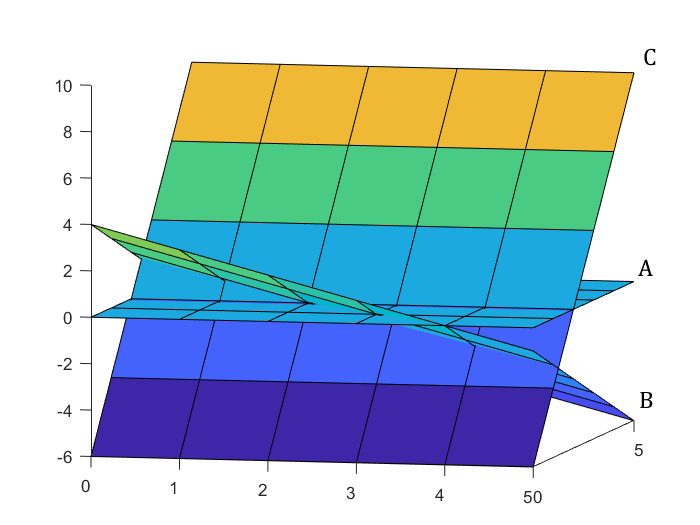
\includegraphics[width=0.9\textwidth]{bounds}
  \caption{Таблиця результатів роботи}
  \label{fig:bounds}
\end{figure}

\subsection{Висновки}
В ході виконання лабораторної роботи було вивчено загальні положення третьої теореми про знаходження ефективних альтернатив для багатокритеріальних задач лінійного (нелінійного) програмування. 
Було вирішено задачу багатокритеріальної оптимізації за допомоги третьої теореми з почерговим вибором кожного критерію вихідної задачі як головного та інших як додаткових обмежень.

Обчислення для кожного критерію виконувались з різноманітними значеннями параметру z, які належали області ZM-1. 
Було помічено, що меншим значенням z відповідали альтернативи, які більшою мірою задовольняли головному критерію, та навпаки. 
Так, для $z = 0$ та $z = 1.75$ відповідними значеннями головного критерію є $f_1(x^*)=4$ (де $\vec{x^*}=(4; 0; 0)$) та $f_1(\vec{x^*})=0.5$ ( де $\vec{x^*}=(0.5; 1.75; 1.75)$) відповідно.

\end{document}

